\chapter{Pomodoro Technique}

\paragraph*{Qu'est ce que c'est?}La technique du pomodoro a été inventée par Fransesco Cirillo. C'est une technique de gestion du temps qui peut être utilisée pour n'importe quelle type de tâche. L'objectif de la technique du pomodoro est de considérer le temps comme un allié dans ce que l'on veut faire et d'améliorer en permanence notre façon de travailler ou d'étudier.

\paragraph*{Que faut-il pour commencer?}
\subparagraph*{Une minuterie de cuisine}
Vous pouvez aussi bien utiliser un pomodoro\footnote{minuterie de cuisine} qu'un timer logiciel. Le régler sur 25 minutes.

\subparagraph*{Une feuille de papier}
Le papier blanc est idéal, c'est encore mieux avec des lignes et le papier à pomodoro pré-imprimé est parfait !

\subparagraph*{Un crayon}
Avoir un gomme est un plus.

\paragraph*{Comment commencer?}
L'unité de travail de base peut être découpée en cinq étapes.
\begin{itemize}
\item{Choisir une tâche à accomplir}
\item{Régler le pomodoro sur 25 minutes}
\item{Travailler sur la tâche jusqu'à ce que le pomodoro sonne et faire une coche en face de la tâche sur la feuille de papier}
\item{Prendre une courte pause (5 minutes)}
\item{Tous les quatre pomodoros prendre une pause plus longue (15-25 minutes)}
\end{itemize}

\subparagraph*{}

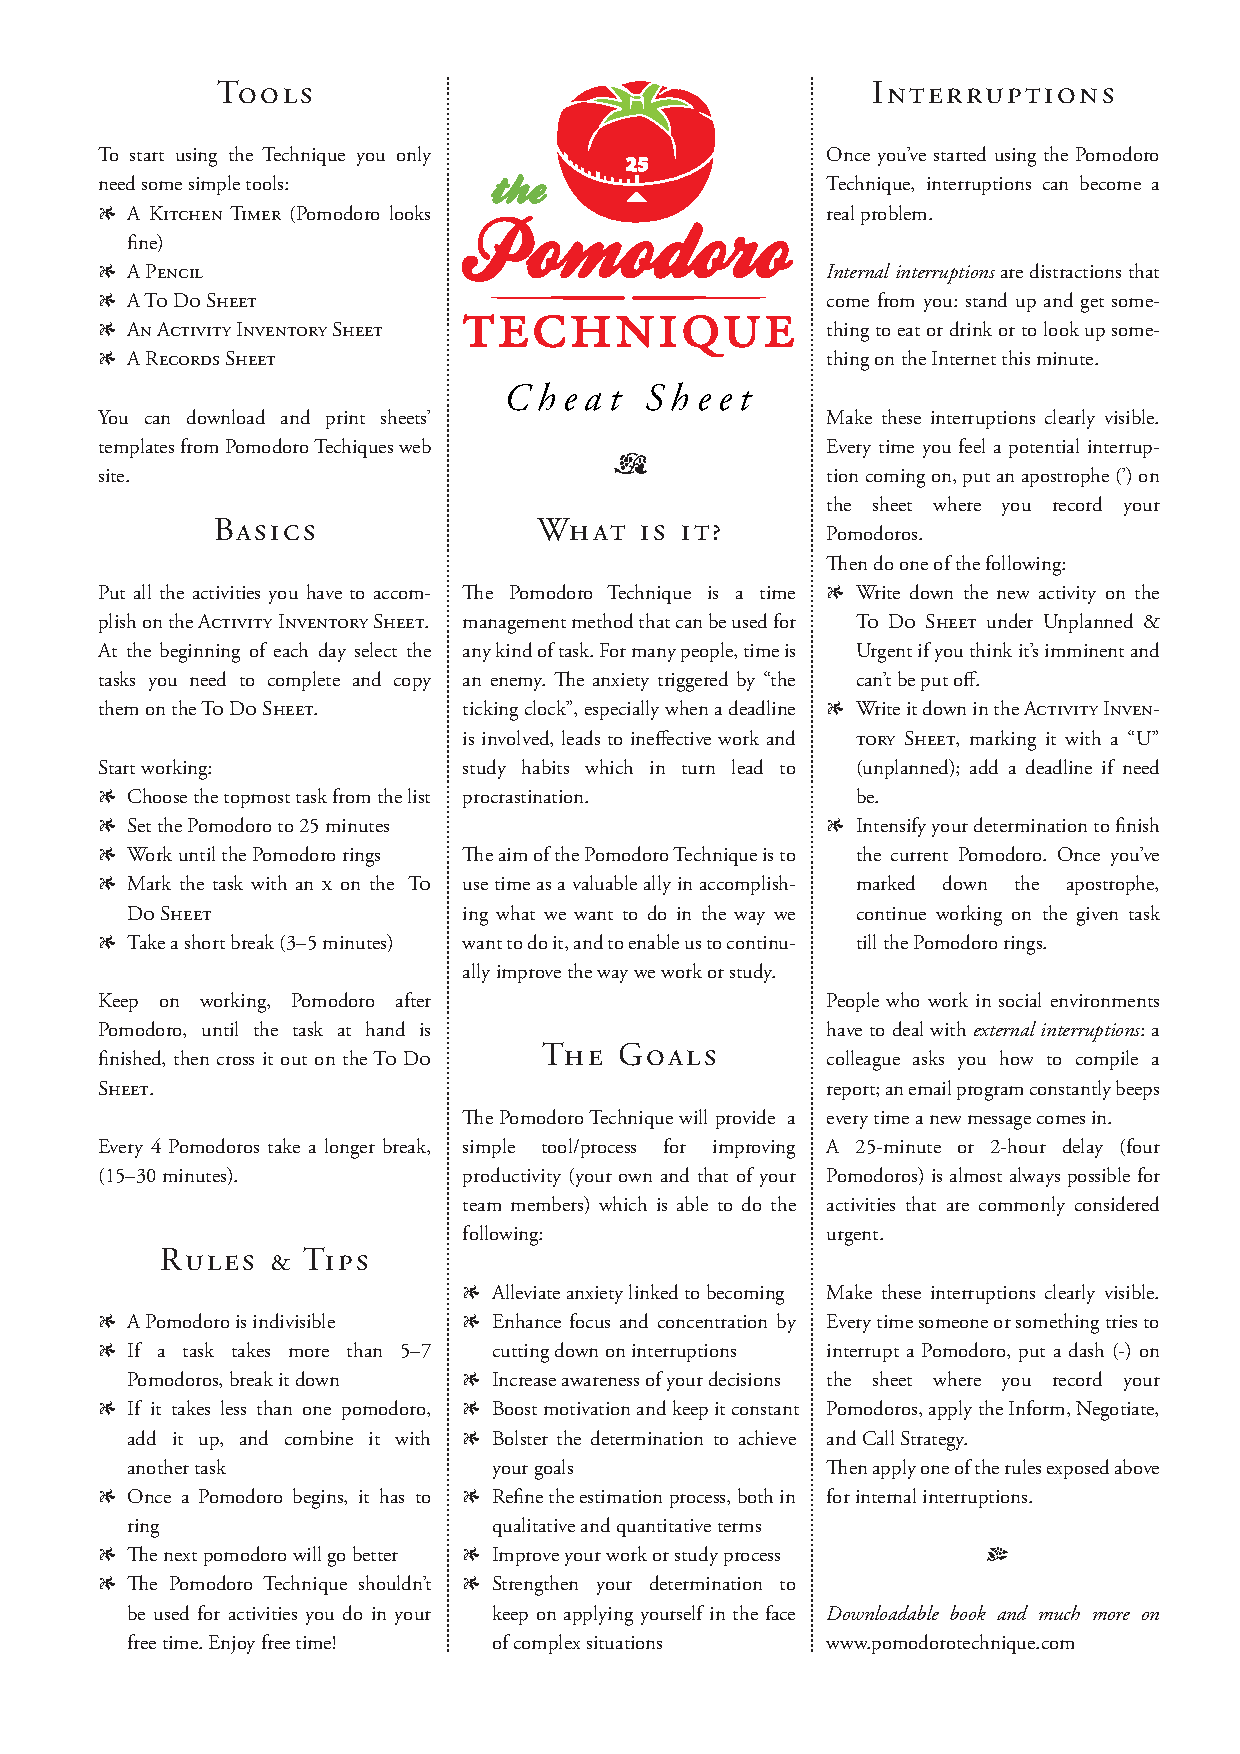
\includepdf[pages=1]{Illustrations/pomodoro_cheat_sheet.pdf} 